\documentclass[11pt]{article}
\usepackage{hyperref}
\usepackage{subfigure}

\usepackage[margin=1in]{geometry}

\usepackage{hyperref}
\hypersetup{unicode=true, colorlinks, breaklinks, citecolor=blue, linkcolor=black}

\usepackage{xltxtra}
\usepackage{booktabs} 
\usepackage{subfigure}
\usepackage{graphicx}
\usepackage{listings}

\lstset{language=Python}

\title{Data Mining Capstone Task 4 and 5}
%\author{Jiacheng Pan}

\begin{document}
\maketitle

\section{Abstract}
In this task, I performed dish / restaurant rankings using the information extracted from reviews.

\section{Implementations}
\subsection{Task 4: Mining Popular Dishes}
In this task, I applied the dish list provided by the staff (\href{https://d28rh4a8wq0iu5.cloudfront.net/dataminingcapstone/Tasks4and5/student_dn_annotations.txt?response-content-type=application%2Foctet-stream&a=1&response-content-disposition=attachment}{link}).
The review data set is all the reviews of "Chinese" category.
Therefore, I choose to rank Chinese dishes.

I used the following formular to compute the score for each dish. This score estimates the popularity and goodness of a particular dish.

$$\log(1 + occurrence) * \frac{(1 + usefulVote) * rate}{1 + usefulVote}$$

Here is my consideration:
\begin{enumerate}
  \item I use the $\log$ term to modify the \emph{Term Frequency}, because I believe that popular dishes are usually mentioned much in reviews, but the final rank order should be determined by not only the popularity, but also the goodness (how delicious, for example) of the dishes.
    Frequently mentioned dishes are roughly equally popular in terms of the occurrence, while the key to distinguish their ranks is their goodness.
    Under such situation, we shouldn't let the occurrence bias the final ranking.
  \item The votes and rating of a review just provide a reliable source of information indicating how meaningful the review is and how good the reviewed restaurant is.
    Presumably, when a review mentions certain dishes, it is likely that the goodness of these dishes correlate with the rating. 
  \item Of course this is merely an inaccurate estimation, since reviewer may find the overall quality of a restaurant is fine, but she may dislike a certain dish which is also mentioned in a positively-ranked review. In such circumstance, current estimation is inaccurate and therefore more sophisticated method should be developed. For example, sentiment analysis over each sentence may yield a better estimation.
    Due to time constraints, I did not implement a complete sentiment analysis estimator.
\end{enumerate}

Figure \ref{fig:dish_rank} shows the ranking result thereby produced.

The height of each bar indicates how frequent the dish is mentioned among all the sampled reviews.
The colour indicates how good the score is -- red means relatively bad, whild green means relatively good. The domain of the colour has been modified to fit the shown data.

I sampled the top 50 dishes.

\vspace{1.5em}
As is shown, top frequent dishes (rice, chicken, beef, etc.) are also very good in review. But less frequent dishes do not necessarily maintains the order of occurrence. For instance, dish \emph{tuna} is more frequently mentioned than \emph{noodle soup}, but judging by the colour, the \emph{noodle soup} is better in quality.

In fact, even though there may be disorder, the differences in score are really small. If we take a look at another visualisation in which height is the score while the colour is the occurrence (figure \ref{fig:dish_rank_1}), we can hardly find any disorder.

\begin{figure}[htp!]
  \centering
  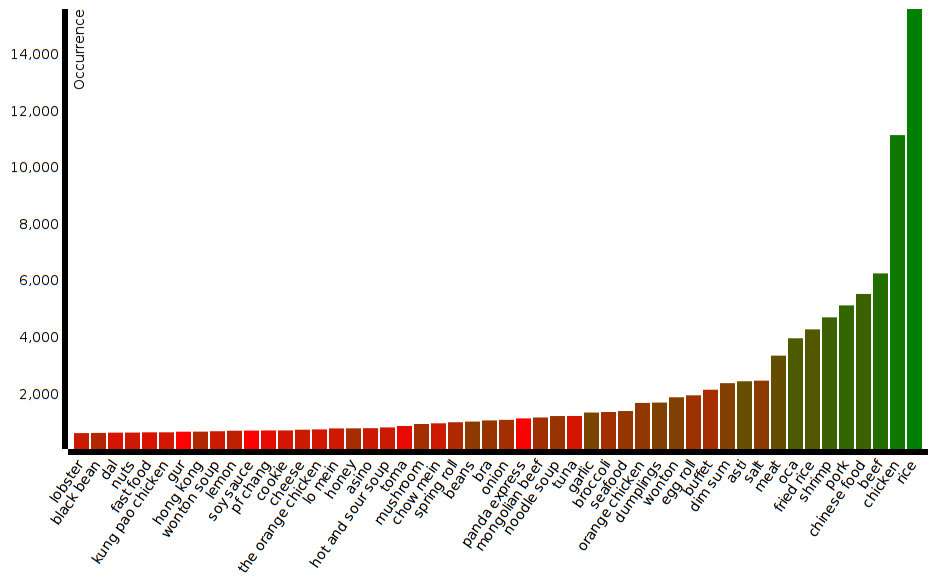
\includegraphics[width=0.8\textwidth]{./img/dish_rank.png}
  \caption{Dish Rank}
  \label{fig:dish_rank}
\end{figure}

\begin{figure}[htp!]
  \centering
  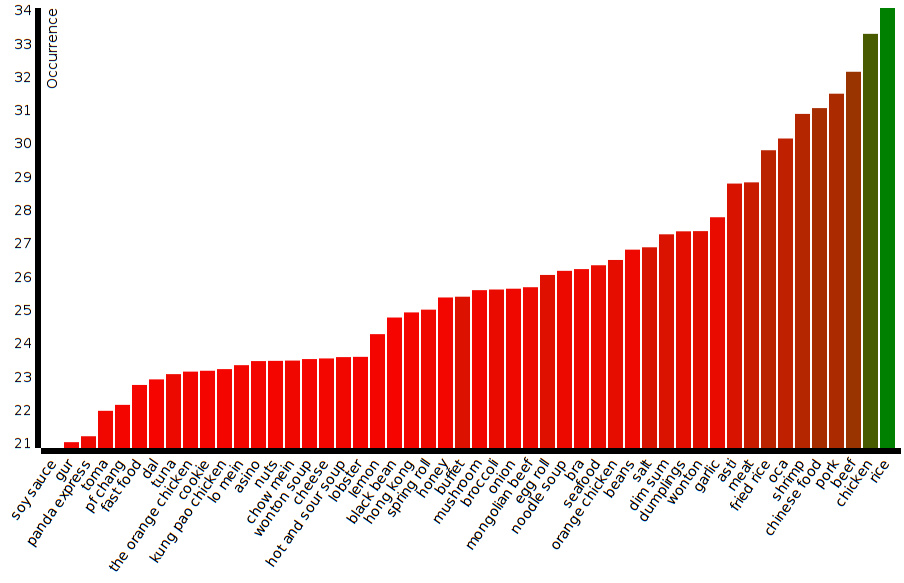
\includegraphics[width=0.8\textwidth]{./img/dish_rank_1.png}
  \caption{Dish Rank with Y as the Score}
  \label{fig:dish_rank_1}
\end{figure}


\subsection{Task 5: Restaurant Recommendation}
In this task, I also applied the dish list provided by the staff, and conducted the ranking of restaurants based on single target dish.

The score, which is used to estimate the goodness of a restaurant and thereby used as the ranking factor, is computed using following formula similar to Task 4:
$$\log(1 + occurrence) * \frac{(1 + usefulVote) * rate}{1 + usefulVote}$$

The difference is that all relevant reviews that mention the target dish, are clustered by the restaurants they are referreing to.
This formula is then applied to each review cluster.
The score yield from each cluster corresponds to the restaurant of the cluster for the target dish.

The score only estimate how good the target dish is in certain restaurants, rather than the overall quality of the restaurants.

\vspace{1.5em}
Figure \ref{fig:rest_rank} shows the ranking result for target dish \emph{beef}.

Similarily, the vertical significance shows how frequent the dish is mentioned among the reviews of a certain restaurant (i.e. the popularity);
and the colour shows how good the dish is computed by the formula above, where red is relatively bad and green good.

As is shown, although the frequency generally correlate with the score, many obvious disorder can be found.
For instance, restaurant \emph{Veggie House} is less popular in terms of the dish frequency than \emph{Noodle Asia}, but the quality of the former one is obviously better than the latter.

\begin{figure}[htp!]
  \centering
  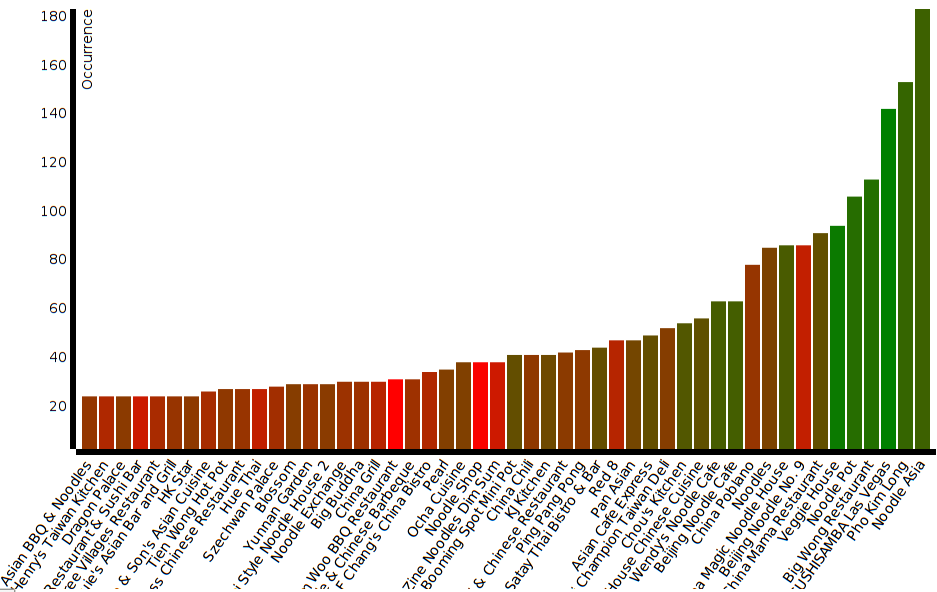
\includegraphics[width=0.8\textwidth]{./img/rest_rank.png}
  \caption{Restaurant Rank for Dish "Beef"}
  \label{fig:rest_rank}
\end{figure}


\end{document}

